%!TeX program = xelatex
\documentclass[12pt,hyperref,a4paper,UTF8]{ctexart}
\usepackage{WHUReport}
\usepackage{mathrsfs}
\usepackage{bookmark}
\usepackage{float} % 引入float包
\usepackage{booktabs} % 导入booktabs包,提供更美观的表格线条
\usepackage{multirow} % 导入multirow包,允许行跨多行
\usepackage{cite} % 导入引用的包,能够使用\cite

% Keywords command
\providecommand{\keywords}[1]
{
  \small	
  % \textbf{\textit{Keywords---}} #1
  \textbf{Keywords:} #1
}
 

%%-------------------------------正文开始---------------------------%%
\begin{document}

%%-----------------------封面--------------------%%
\cover

%%------------------摘要-------------%%
\begin{abstract}
    全球导航卫星系统(GNSS)在城市环境中的应用面临着多路径效应、信号遮挡和电磁干扰等挑战,这些问题严重影响了GNSS的定位精度和可靠性。本课程报告综合回顾了城市环境下GNSS抗差技术的最新研究进展,特别关注了多路径效应的抑制方法、信号遮挡的解决方案以及抗干扰技术的发展。在众多抗差方法中,本报告重点介绍了四种常见技术:最小二乘残差法、粗差拟准检定法、众数投票法和RANSAC方法。最小二乘残差法通过统计假设检验来检测并剔除粗差;粗差拟准检定法通过解算秩亏方程组来识别和修正粗差;众数投票法利用已知的精确信息来发现单历元粗差;而RANSAC方法则是一种迭代方法,用于从包含异常值的数据中估计数学模型参数,特别适用于数据包含显著噪声或异常值时的鲁棒性拟合。尽管已有显著进展,但仍存在挑战,未来的研究需进一步探索多路径效应的精确建模、信号遮挡情况下的高精度定位技术以及抗干扰技术的优化。此外,随着人工智能和机器学习技术的发展,这些技术在GNSS抗差技术中的应用也显示出巨大潜力。本报告总结了当前的研究进展,并对未来的研究方向提出了展望。
\end{abstract}

\keywords{城市环境,最小二乘残差法,粗差拟准检定法,众数投票法,RANSAC方法}
\thispagestyle{empty} % 首页不显示页码

%%--------------------------目录页------------------------%%
\newpage
\tableofcontents

%%------------------------正文页从这里开始-------------------%
\newpage

%%可选择这里也放一个标题
%\begin{center}
%    \title{ \Huge \textbf{{标题}}}
%\end{center}


\section{引言}
随着全球定位系统(Global Navigation Satellite System, GNSS)技术的不断发展,GNSS在各个领域的应用越来越广泛,尤其是在城市环境中的应用。然而,城市环境中的复杂电磁环境和建筑物密集分布对GNSS信号的接收和定位精度提出了严峻挑战。本次课程报告通过文献调研,探讨和总结了近年来在城市环境下GNSS抗差技术的研究进展。

城市环境中的GNSS应用面临的主要挑战包括多路径效应、信号遮挡和电磁干扰等问题。多路径效应是指GNSS信号在传播过程中受到建筑物、地面等反射物的影响,导致信号到达接收机时出现多个路径,从而影响定位精度。信号遮挡是指由于高楼大厦等障碍物的存在,导致GNSS信号无法直接到达接收机,影响定位性能。电磁干扰是指城市环境中存在大量的电磁干扰源,如无线电发射设备、移动通信基站等,对GNSS信号的接收造成干扰。


\section{文献综述}
近年来,针对城市环境下GNSS抗差技术的研究取得了显著进展。本次课程报告从多路径效应、信号遮挡和抗干扰技术三个方面的相关文献进行详细阐述。

\subsection{多路径效应}
在城市环境中,GNSS信号的多路径效应是影响定位精度的主要因素之一\cite{fan2010}。多路径效应是指GNSS信号在到达接收机天线之前,因反射、折射或散射而产生的多条信号路径,这些信号的叠加会导致定位误差。

天线设计优化作为抑制多路径效应的重要手段之一,已经在多个研究中得到验证和应用。通过优化天线的设计,可以有效减少多路径信号的接收,提高定位精度。
王春华等\cite{wang2014}介绍了一种具有多径抑制效应的3D扼流圈天线,该天线可以同时应用于GNSS卫星导航系统的G1和G2两个频段。试验结果表明,该天线对多径信号具有较强的抑制能力,且相位中心稳定,具有较强的抗干扰能力。
Boccia等\cite{boccia2001}提出并设计了一种高性能双频微带天线,该天线设计用于全球定位系统,特别强调了对多路径信号的优越抑制能力。通过优化天线几何结构,实现了在两个GPS频率(L1和L2)上的高性能操作。
Jan和Wong\cite{jan2000}描述了一种用于双频圆极化辐射的探针馈电堆叠微带天线。通过适当选择两个不同轴比的椭圆贴片,并在两个贴片之间引入一个小的空气间隙层,可以实现双频圆极化辐射。
李运志等\cite{li2011}设计了一种单馈电层叠贴片天线,该天线结合调谐枝节技术,设计了可工作于L1/L2频段的多模GNSS圆极化天线。通过在上层方形贴片上插入长度不同的枝节,实现了GNSS高频段的圆极化,同时在下层方形贴片插入枝节以满足GNSS低频点的右旋圆极化工作模式。
王世超等\cite{wang2013}在其研究中分析了GNSS多路径效应对车辆定位精度的影响,并提出了几种抑制GNSS多路径效应的方法,包括天线设计优化、数据处理算法改进、多传感器融合定位和基站数据辅助。这些方法可以有效地降低多路径效应带来的定位误差,提高定位结果的准确性和稳定性。

此外信号处理算法的改进也是抑制多路径效应的重要方法。黄声享等\cite{huang2005}分析了GPS多路径效应的特性,并结合动态变形监测的特点,提出了采用滤波与周日位置求差相结合的方法进行数据处理。研究表明,这种方法显著提高了GPS动态监测的精度,尤其是在垂直方向的精度改善明显。
王世超等\cite{wang2013}探讨了多路径效应对车辆定位精度的影响,提出了几种抑制GNSS多路径效应的方法,包括信号处理算法的改进。研究中指出,使用卡尔曼滤波器和粒子滤波器等先进的信号处理算法,可以有效降低多路径信号的影响,从而提高定位精度。
朱彬等\cite{zhu2021}则提出了一种基于非监督学习的信号处理方法,通过对GNSS信号进行聚类分析,能够有效区分视线信号(LOS)和非视线信号(NLOS),从而减小多路径效应对定位精度的影响。研究表明,采用k-means++和高斯混合模型(GMM)等方法,可以显著提高定位精度,尤其是在复杂城市环境中。
范晓燕等\cite{fan2010zhou}综述了多路径效应产生的原理及其对GPS测量精度的影响,强调了信号处理技术在减小多路径误差中的重要性。文中采用信号分离技术和滤波技术可以有效降低多路径信号的影响,提高定位结果的可靠性。最后,蒋光伟等人通过对GNSS数据的分析,探讨了多路径效应与数据质量之间的关系,提出了基于信噪比和伪距残差的信号处理方法,以提高数据质量和定位精度。研究结果表明,改进的信号处理算法能够有效抑制多路径效应,提高定位精度\cite{jiang2018}。

多路径效应建模是研究GNSS信号多路径效应的重要手段之一,能够有效帮助理解和减小多路径信号对定位精度的影响。殷海涛和熊永良\cite{yinhaitao2003}在其研究中全面论述了GPS测量中多路径效应的产生原理,并简要介绍了近年来国内外减弱和消除多路径效应的方法及手段,强调了多路径建模在这一过程中的关键作用。
范晓燕和周乾\cite{fanxiaoyan2010}指出,多路径效应不仅是影响GPS测量精度的主要误差源,而且其复杂性使得建模成为一项重要的研究任务。通过建立多路径效应模型,研究者能够更好地理解多路径信号的特性和影响规律,从而为后续的误差修正提供理论基础。
黄声享等\cite{huangshengxiang2005}结合GPS动态变形监测的特点,提出了采用滤波与周日位置求差相结合的方法进行数据处理,研究结果表明,多路径误差具有较强的周日重复性。在此基础上,他们强调了通过多路径建模来识别和消除多路径效应的重要性,指出在动态监测中,合理的建模策略能够显著提高三维位置精度,达到毫米级。
蒋光伟等\cite{jiangguangwei2018}通过对GNSS数据的分析,探讨了多路径效应与数据质量之间的关系,提出了一种基于信噪比和伪距残差的多路径建模方法。该方法通过建立数学模型来纠正多路径效应,从而提高定位精度,研究结果表明,改进的信号处理算法能够有效抑制多路径效应,提高GNSS定位的可靠性。

\subsection{信号遮挡}
城市环境中的高楼大厦和其他障碍物会导致GNSS信号的遮挡,影响定位性能。为解决这一问题,研究人员提出了多传感器融合技术、辅助定位技术和信号预测模型等方法。

多传感器融合技术通过融合多种传感器数据,如惯性测量单元(IMU)、Wi-Fi和蜂窝网络信号,可以在信号遮挡情况下提供可靠的定位信息。
研究表明,惯性测量单元(IMU)可以提供高频率的运动信息,帮助补充GNSS信号在遮挡时的不足。IMU通过测量加速度和角速度,能够实时估计设备的运动状态,从而在GNSS信号丢失时维持定位能力\cite{2019li}。此外,Wi-Fi和蜂窝网络信号的结合使用也能有效提高定位的鲁棒性。文献中指出,Wi-Fi信号在室内环境中具有较强的穿透能力,可以作为GNSS信号的有效补充,尤其是在城市高楼林立的环境中\cite{2020zhang}。
张伟等\cite{2020zhang}提出了一种基于多传感器融合的定位系统,该系统结合了GNSS、IMU和Wi-Fi信号,通过卡尔曼滤波算法对传感器数据进行融合,显著提高了在信号遮挡情况下的定位精度和可靠性。李明等\cite{2019li}研究了基于IMU和GNSS的组合定位方法,结果表明,在GNSS信号受到遮挡的情况下,IMU能够有效地维持定位精度,减少定位漂移。
多传感器融合技术在信号遮挡情况下提供可靠定位信息的研究中,磁场传感器的应用逐渐受到重视。磁场传感器能够提供环境的独特特征,尤其是在室内环境中,结合惯性测量单元(IMU)和Wi-Fi信号,可以显著提高定位的精度和可靠性。

而磁场传感器可以有效补充GNSS信号在遮挡时的不足。Wang等\cite{2018wang}提出了一种基于智能手机传感器的磁场室内定位系统,通过分析环境中的磁场变化,结合其他传感器数据,能够在复杂环境中实现高精度定位。此外,Liu等\cite{2017liu}开发了一种基于磁场的室内定位系统,利用智能手机传感器的磁场数据,结合卡尔曼滤波算法,显著提高了定位精度。
Al-Muhtadi等\cite{2020almuhtadi}探讨了将磁场传感器与Wi-Fi信号结合的多传感器融合方法,研究结果表明,该方法在信号遮挡情况下能够有效提高定位的鲁棒性和精度。通过融合磁场、IMU和Wi-Fi信号,这些研究展示了多传感器融合技术在解决信号遮挡问题中的潜力。

辅助定位技术利用实时动态差分(RTK)和精密单点定位(PPP)等高精度定位技术,可以在信号遮挡情况下提供高精度定位服务。
实时动态差分(RTK)技术通过建立基准站和移动站之间的差分关系,能够在短时间内提供厘米级的定位精度。研究表明,RTK技术在信号遮挡时仍能保持较高的定位精度,尤其是在基准站与移动站之间的视线信号良好时,定位结果的可靠性显著提高。张伟等\cite{2018zhang}提出了一种基于RTK的定位系统,该系统在城市环境中通过优化基准站的布设和信号处理算法,有效减小了信号遮挡对定位精度的影响。

精密单点定位(PPP)技术则通过使用精确的卫星星历和大气模型,能够在无基准站的情况下实现高精度定位。PPP技术尤其适用于信号遮挡较严重的环境,研究表明,该技术在城市峡谷等复杂环境中能够提供亚米级的定位精度。张小红等\cite{zhangxiaohong}研究了PPP在信号遮挡情况下的应用,结果表明,通过引入精确的气象数据和多路径模型,PPP技术能够有效提高定位精度和可靠性。

信号预测模型通过对历史信号数据进行分析和建模,可以在信号遮挡情况下预测信号的变化趋势,从而提高定位精度。近年来,信号预测模型在GNSS领域的应用取得了显著进展。LI Wei等\cite{10}提出了一种基于Prophet-RF模型的GNSS垂直坐标时间序列预测方法。该方法结合了Prophet模型和随机森林(RF)的特点,有效解决了Prophet模型对时间序列非线性部分预测能力弱的问题,具有较强的鲁棒性。通过对BJFS站连续观测数据的分析,设计了多种组合方案,测试了组合模型的适用性和准确性。实验结果表明,Prophet-RF复合模型在表示垂直坐标时间序列的变化趋势和获得更准确的预测数据方面优于单一的Prophet模型。
CAI\ Xi等\cite{11}提出了一种快速预测城市峡谷环境下GNSS卫星可见性的方法。该方法通过分析三角面的法向量方向、三角面与用户之间的相对位置以及相邻两个时刻之间的遮挡关系,减少了计算负担,缩短了计算时间。模拟结果表明,该方法的交集计算次数仅为传统方法的7.21\%,计算时间减少了22.38\%,平均相对误差仅为1.89\%,具有更高的计算效率和准确性。

\subsection{抗干扰技术}
城市环境中的电磁干扰源众多,对GNSS信号的接收造成干扰。近年来,抗干扰技术取得了显著进展,包括自适应滤波技术、干扰检测与抑制技术和抗干扰天线设计等。

自适应滤波技术通过实时检测和抑制干扰信号,提高定位精度。自适应滤波技术因其能够实时检测和抑制干扰信号而成为该领域的研究热点。这种技术通过动态调整滤波器参数,有效分离接收信号中的有用信号和干扰信号,从而提高GNSS接收机的定位精度。
自适应滤波技术的研究进展表明,该技术能够有效地提高GNSS系统的抗干扰能力。王建民在其综述文章中详细讨论了自适应滤波技术的原理和应用,强调了其在实时检测和抑制干扰信号方面的重要性\cite{王建民2010自适应滤波技术综述}。徐新龙在其博士论文中深入研究了自适应滤波算法及其应用,为自适应滤波技术的发展提供了理论基础\cite{徐新龙0自适应滤波算法及其应用研究}。
在GNSS领域,梅林和鲍尧提供了GNSS干扰分析及抗干扰技术的综述,特别强调了自适应滤波技术在抗干扰中的应用\cite{梅林2021GNSS}。王晓燕等人进一步探讨了GNSS干扰和欺骗检测技术,包括自适应滤波技术的应用\cite{XXCN202312003}。
胡祥祥等人提出了一种基于自适应优化选择-抗差自适应卡尔曼滤波混合模型的GNSS+5G组合定位方法,该方法通过自适应滤波技术提高了定位精度和系统的抗干扰能力\cite{CHTB202407005}。尹继东和冯雪峰在他们的综述文章中也对GNSS抗干扰技术进行了全面的总结,包括自适应滤波技术的应用\cite{尹继东2020GNSS}。

干扰检测与抑制技术通过有效识别和消除干扰信号,保障GNSS信号的正常接收。王鹏宇等人提出了一种基于卷积神经网络的干扰识别算法,该算法通过联合多域特征提取,显著提升了在低信噪比下分类准确率,增强了干扰特征的抗噪性能\cite{wang2023interference}。这一研究为GNSS干扰识别提供了新的技术手段,有助于提高系统的抗干扰能力。
征惠玲在其研究中分析了当前无线通信抗干扰主要手段存在的不足,并指出多维抗干扰和认知抗干扰是当前研究的主要热点\cite{zheng2023wireless}。该文献进一步介绍了国外近年提出的无线通信抗干扰新概念和技术及其研究情况,为GNSS抗干扰技术的发展提供了宝贵的参考。
梅林等人提供了GNSS干扰分析及抗干扰技术的综述,包括干扰信号的检测与测向,为GNSS信号的正常接收提供了重要的技术支持\cite{梅林2021GNSS}。

抗干扰天线设计通过优化天线结构和材料,提高天线的抗干扰能力。通过精心设计的天线结构和材料选择,可以有效降低外部干扰对GNSS信号的影响。
在抗干扰天线设计方面,有研究提出了采用功率倒置算法的调零天线阵,适用于强干扰环境,并讨论了天线单元设计及布阵形式对于调零效果的影响\cite{147}。此外,基于数字孪生的天线结构优化设计也被提出,通过改变天线方向性的设计,对天线的辐射特性参数进行优化,以提高信号质量验证及开发创新\cite{148}。这些研究为抗干扰天线设计提供了新的思路和方法。
在材料科学方面,基于电磁超材料的抗干扰天线设计也取得了进展。这种天线设计能有效提高天线的抗干扰能力,通过特定的结构设计,实现了对干扰信号的有效抑制\cite{150}。北斗抗干扰天线的设计与实现也是该领域的一个重要成果,研究结果表明,采用空时自适应调零技术的B3天线阵列能有效提高天线的抗干扰能力\cite{154}。

\section{常见方法}
近年来,针对城市环境下GNSS抗差技术的研究提出了多种方法。由于篇幅限制,本次课程报告仅从城市环境下的粗差探测和识别角度进行一个方法的阐述和分享。
在对城市环境下的测量数据进行处理处理时,关于粗差探测和剔除的方法很多,本报告将对诸多方法中比较常见和实用的方法进行详细阐述,包括最小二乘残差法、粗差拟准检定法、众数投票法和最新的RANSAC方法等。
\subsection{最小二乘残差法}
最小二乘残差法是由巴尔干提出的,其基本思想是假定平差系统只有一个观测存在粗差,并纳入函数模型,用统计假设检验方法检测粗差并剔除粗差。剔除含有粗差的观测值后,建立新的平差系统,若还存在粗差,在假设只存在一个粗差,逐次不断进行,直至判断不再含有粗差。

设有误差方程为:
\begin{equation}
\mathbf{V} = \mathbf{A} \mathbf{\hat{X}} + \mathbf{l}
\label{(1)}
\end{equation}
其最小二乘解为
\begin{equation}
\mathbf{\hat{X}} = \left(\mathbf{A}^T \mathbf{P} \mathbf{A}\right)^{-1} \mathbf{A}^T \mathbf{P} \mathbf{l} = \mathbf{Q}_{\hat{\mathbf{X}} \hat{\mathbf{X}}} \mathbf{A}^T \mathbf{P} \mathbf{l}
\end{equation}
已知平差系统的函数模型为
\begin{equation}
\mathbf{l} = \mathbf{A} \mathbf{X} + \Delta
\end{equation}
代入误差方程(\ref{(1)})得
\begin{equation}
\mathbf{V} = \mathbf{A} (\mathbf{\hat{X}} - \mathbf{X}) - \Delta
\end{equation}
因为
\begin{equation}
\mathbf{\hat{X}} - \mathbf{X} = \left(\mathbf{A}^T \mathbf{P} \mathbf{A}\right)^{-1} \mathbf{A}^T \mathbf{P} \Delta
\end{equation}
所以
\begin{equation}
\mathbf{V} = \left[\mathbf{A} \left(\mathbf{A}^T \mathbf{P} \mathbf{A}\right)^{-1} \mathbf{A}^T \mathbf{P} - \mathbf{I}\right] \Delta
\end{equation}
当 $\Delta$ 为偶然误差时, $E(\Delta)=0$,所以可以得不含粗差影响的 $\mathbf{V}^{\prime}$ ,其期望为
\begin{equation}
    E(\Delta) = 0 
\end{equation}
方差为
\begin{equation}
D(\mathbf{V}) = \sigma_0^2 \mathbf{Q}_{\mathbf{V} \mathbf{V}}
\end{equation}
向量$\mathbf{V}$为正态向量。

对于残差 $\mathbf{v}_t$, 其满足$\mathbf{v}_t \sim N\left(0, \sigma_0^2 \mathbf{Q}_{\mathbf{V} \mathbf{V}}\right)$ 变量, 这是在不含粗差情况下成立。如果含有粗差影响, 这时,第 $i$ 观测值改正数
\begin{equation}
\mathbf{v}_t^{\prime} = \mathbf{v}_t + \mathbf{v}_{\mathbf{\varepsilon}_t}
\end{equation}
其期望为$E\left(\mathbf{v}_t^{\prime}\right) = \mathbf{v}_{\mathbf{\varepsilon}_t}$
不等于零。为了检验 $\mathbf{v}_{\mathbf{\varepsilon}_t}$ 是否存在, 可作如下假设检验:

原假设: $\quad H_0: E\left(v_t\right)=0, H_1: E\left(v_t\right) \neq 0$

检验统计量采用正态分布标准化残差(改正数):
\begin{equation}
    \mathbf{W}_i=\frac{\left|v_t\right|}{\sigma_{r_i}}=\frac{\left|v_t\right|}{\sigma_0 \sqrt{Q_{v_t} r_i}}=\frac{\left|v_t\right|}{\sigma_{1,} \sqrt{r_i}}
\end{equation}
原假设 $H_0$ 成立时, $W_1 \sim N(\mu, \sigma)$ 。

首先对实测数据进行数理统计,建立实测数据的分布模型, 然后将模型归化到标准正态分布中去, 最后选定适当的显著水平 $a$, 查得标准正态分布的分位值 $u_{a/ 2}$ 。

进行检验, 如果 $\mathbf{W}_1<u_{a / 2}$则接受 $H_0$, 可认为 $E\left(v_r\right)=0, \mathbf{V}_r$ 不受粗差影响,否则可判断存在粗差影响。

\subsection{粗差拟准检定法}

粗差拟准检定法以观测值的真误差为研究对象,通过附加“拟准观测的真误差估值范数极小”的条件,解算真误差与观测量之间的秩亏方程组,求出真误差估值,然后比较真误差估值大小,判断出可能存在的粗差\cite{2004041259nh}。该方法是一种选群拟合,可以同时辨识、定位观测数中多个粗差,并能估计粗差大小和精度。

载波相位观测方程的线性化为:
\begin{equation}
    \begin{aligned}
        \widetilde{D}_t^j= & \left(D_t^j(t)\right)-\left[k_t^j(t) \delta X_t^j+l_t^j(t) \delta Y_t+m_t^j(t) \delta Z_t\right]+ \\
        & \delta I_t^j(t)+\delta T_t^j(t)+c \delta t_t-c \delta t^j-\lambda N_t^j\left(t_0\right)
    \end{aligned}
\end{equation}
上式可以简化式为:
\begin{equation}
    A \delta X+B \cdot N=L+\Delta 
\end{equation}
写成矩阵格式为:
\begin{equation}
\left[\begin{array}{ll}
A & B
\end{array}\right] \cdot\left[\begin{array}{c}
\delta X \\
N
\end{array}\right]=L+\Delta
\label{(13)}
\end{equation}
上式中: $A_t$ 为 $n \times 3$ 的系数矩阵, ($n$ 为该测站观测值个数), $N$ 为 $k$ 维整周模糊度向量, $L_t$ 为 $n$ 维观测值向量, $\Delta$ 为 $n$ 维真误差向量, P 为权阵, 令 $C=\left[\begin{array}{ll}A & B\end{array}\right]$, $G=\left[\begin{array}{ll}\delta X & N\end{array}\right]^T$,则观测方程可以写为:
\begin{equation}
    C \cdot G=L+\Delta
\end{equation}
上式中 C 为 $n \times(k+3)$ 维系数矩阵, $G$ 为 $k+3$ 维待估参数向量, 平差因子阵为 $J=C\left(C^T P C\right)^{-1} C^T P$, 其正交补矩阵为 $R=I-J $,$I$ 为 $n$ 维单位阵。由公式(\ref{(13)})得:
\begin{equation}
    R \Delta=-R L
    \label{(15)}
\end{equation}
由于矩阵 $R$ 秩亏, 求得的真误差估值 $\Delta$ 不唯一, 但可以选出 $r(>k+3)$ 个拟准观测,然后附加 "拟准观测真误差 $\Delta_r$ ,范数极小" 的条件, 即
\begin{equation}
    \|\Delta_r\|^2_P=\Delta_r^T P \Delta=\min
\end{equation}
此时对应的系数阵为 $C_r$, 取
$
H=\left(0, C_r^T\right)^T, \quad P=\left[\begin{array}{ll}
0 & 0 \\
0 & P_r
\end{array}\right]
$
则由方程 (\ref{(15)}) 求解真误差估值为:
\begin{equation}
    \Delta=-\left(R^T R+P H^T H P\right)^{-1} \cdot R^T R L
\end{equation}


通过初选, 复选拟准观测求得 $\Delta$, 根据其呈现明显分群特征,确定粗差的位置。
\subsection{众数投票法}
"众数投票" 法(Majority Voting)是著名的GPS定位、定轨软件Bernese 5.0 中提出的一种粗差探测方法, 其基本原理是在消电离层组合的码观测方程中如果已知精密卫星星历、卫星钟差和接收机位置的先验三维坐标, 则方程中只有接收机钟差一个需要求解参数, 如果已知的信息比较准确, 则同一历元对不同卫星的接收机钟差应在一定的范围内变化, 据此我们可以发现单历元粗差。

如果已知第 $i$ 历元卫星三维位置 $\left(x_j, z_j, z_j\right)$, 该历元对应第 $j$ 颗卫星钟差为 $T^j$, 历元接收机先验位置 $(X, Y, Z), \widetilde{P}$, 为对应 $j$ 颗卫星双频 P 码的消电离层组合的观测值减计算值所的向量, 则该历元每颗卫星对应的接收机钟差为:
\begin{equation}
    t_j=\frac{\tilde{p}_j-\sqrt{\left(x_j-X\right)^2+\left(y_j-V^2+\left(z_j-Z\right)^2\right.}+c T^j}{c}
\end{equation}

从数理统计的观点看, GPS观测值服从正态分布,所以对应两颗观测卫星 $k$ 和 $j$ 的接收机钟差改正数应该以相同的概率落到一定的区间内。在所有卫星对应的接收机钟差 $t_j(j=1,2, \cdots, n)$ 之间相互求差, 其中 $n$ 为该历元观测的卫星总数。并判断差值绝对值是否小于 $a \sigma_{ionosphere-free}$ :
\begin{equation}
    \begin{cases}
        & \Delta t_{j, k}=\left|t_k-t_j\right| \leq a \sigma_{ionosphere-free } \\
        & (k=1,2, \cdots, n, j=1,2, \cdots, n)
    \end{cases}
\end{equation}
上式中: $\sigma_{ionosphere-free }$ 为码消电离层组合观测值的标准差, $\sigma$ 为码观测值的标准差, $a$ 为系数, 其中
\begin{equation}
    \sigma_{ionosphere-free }=\sqrt{2} \sigma
\end{equation}

对于某一 $t_k$, 将所有满足条件的 $t_j$ 都放到 $t_k$ 这一组,这样,我们就得到 $n$ 组不同的接受值。然后我们选取接受值最多的一组, 然后求取该组接收机钟差的平均值 $\bar{t}$ 和标准差 $\sigma_t$ 。最后根据对应不同卫星接收机钟差与所求绝对值之差判断其对应的观测值是否为粗差。如果: $\left|t_j-\bar{t}\right| \leq \beta \sigma_t$, 则对应 $j$ 卫星的观测值没有粗差。如果: $\left|t_j-\bar{t}\right|>\beta \sigma_t$, 则对应 $j$ 卫星的观测值有

粗差,应予以剔除。对于多历元粗差探测,依据是利用相邻历元相位差分方程中的接收机钟差之差应该也在一定范围内变化。

通过上面对众数投票法原理的分析,在数据粗差探测过程中有三个关键参数的选取:其一是测站接收
机三维位置,其二是在首次数据筛选中$a$的选取,其三是最后选取粗差观测值中$\beta$的选取。针对上述三个
关键问题,采取了如下的改进措施,其一是测站先验信息选取国际数据处理中心提供的跟踪站三维坐标其二对于参数$a$和$\beta$进行迭代选取,不断调整拒绝域阀值,尽量减少取值不合理造成部分观测值被删除。对于有异常的观测值采用迭代最小二乘过程确定其是否为粗差\cite{WHCH200203003}。

\subsection{RANSAC方法}
RANSAC(Random Sample Consensus)算法是一种用于从包含异常值的数据中估计数学模型参数的迭代方法。该方法特别适用于数据包含显著噪声或异常值时的鲁棒性拟合。

1. \textbf{模型拟合}:对于给定的数据点集 \( D \) 和随机选择的样本 \( S \),模型 \( M \) 的参数 \( P \) 可以通过最小化误差函数 \( E \) 来估计:
\begin{equation}
    P = \arg\min_{P} E(S, M(P, S))
\end{equation}
其中,\( E \) 表示误差函数,它衡量模型 \( M \) 与样本 \( S \) 的拟合程度。

2. \textbf{误差计算}:对于每个数据点 \( x_i \),其与模型 \( M \) 的误差 \( e_i \) 可以表示为:
\begin{equation}
    e_i = |x_i - M(P, x_i)|
\end{equation}
或者对于回归问题,误差可能使用其他度量,如平方误差:
\begin{equation}
    e_i = (y_i - M(P, x_i))^2
\end{equation}

3. \textbf{共识集合}:共识集合 \( C \) 包含所有满足误差阈值 \( e \) 的数据点:
\begin{equation}
    C = \{ x_i \in D \mid e_i \leq e \}
\end{equation}

4. \textbf{迭代选择}:在每次迭代中,算法随机选择样本 \( S \) 并计算共识集合 \( C \)。算法重复这一过程 \( k \) 次,其中 \( k \) 可以通过以下公式估算:
\begin{equation}
    k = \left\lceil \frac{\log(1 - p)}{\log(1 - t^s)} \right\rceil
\end{equation}
其中,\( p \) 是所求模型被接受的概率(通常设置为 0.99),\( t \) 是模型被接受所需的最小共识比例(即 \( C \) 的大小占 \( D \) 的比例),\( s \) 是模型估计所需的最小样本数。

5. \textbf{最终模型选择}:在 \( k \) 次迭代后,选择具有最大共识集合的模型参数作为最终模型:
\begin{equation}
    P_{\text{final}} = \arg\max_{P} |C|
\end{equation}

具体到GNSS在城市环境下的抗差情况,可以用以下图片加以表述RANSAC方法在GNSS抗差领域的应用\cite{Ding_long}:
\begin{figure}[H]
    \centering
    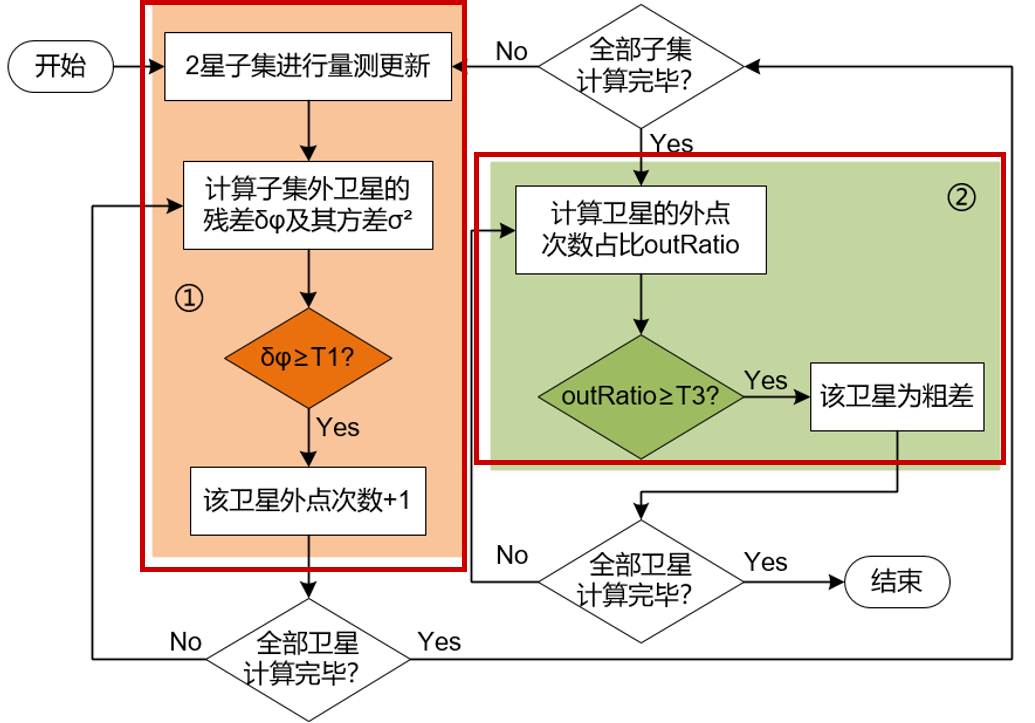
\includegraphics[width=0.8\textwidth]{figures/RANSAC方法.png}
    \caption{RANSAC方法示意图}
    \label{figure-ransac}
\end{figure}
    
目前针对RANSAC粗差探测算法的研究主要集中在如何提高运算效率、如
何有效提取外点等。针对前者,主要通过子集预筛选降低子集数量;针对后者,
主要从阈值和代价函数等方面入手。在GNSS/INS组合导航系统中,RANSAC算
法的应用较少,有少数文献将其应用于松组合中\cite{Sunran2021},
但本质仍然是纯GNSS的完好性监测,没有发挥出INS的作用。而如果将
RANSAC 算法用于紧组合粗差探测,明显的优势为:在INS的辅助下,每个子
集仅需要2颗卫星,子集筛选方法也更加简单有效;同时,如果INS预测值出现
问题,会导致外点数量急剧增加,因此这种方法也可以简单实现对INS的完好性
监测。

\section{算法运行结果}
通过选取实测数据,分别采用以上方法进行检测和处理。
首先选取2009年10月27号IGS跟踪站观测数据模拟粗
差,观测数据采样间隔为30s,卫星高度角为15°,然
后利用上述方法进行检测和处理。并且采取如下的解算方案:
利用上述三种方法探测及剔除单历元下
一个和多个粗差;表示形式为“模拟粗差/卫星代号”\cite{8},
分别是单个粗差60m/5,两个粗差-5m/3、3m/5
算例处理结果如下表:
\begin{table}[h]
    \centering
    \caption{粗差探测及剔除方法的比较}
    \label{tab:comparison}
    \begin{tabular}{ccccccc}
    \toprule
    \multirow{2}{*}{方法} & \multirow{2}{*}{模拟粗差/观测值} & \multirow{2}{*}{判定情况} & \multirow{2}{*}{参数} & \multicolumn{2}{c}{中误差} \\
    \cmidrule(lr){5-6}
     &  &  &  & 剔除前 & 剔除后 \\
    \midrule
    \multirow{7}{*}{最小二乘残差法} & 1 & 无 & \multirow{2}{*}{$\delta x$ 参数} & \multirow{2}{*}{14.4784} & \multirow{2}{*}{0.0004} \\
     & 2 & 无 &  & &  \\
     & 3 & 无 & \multirow{2}{*}{$\delta y$ 参数} &\multirow{2}{*}{17.0159}  & \multirow{2}{*}{0.0004} \\
     & 4 & 无 &  & &  \\
     & 60m/5 & 有/剔除 & \multirow{2}{*}{$\delta z$ 参数} &\multirow{2}{*}{63.3577}  & \multirow{2}{*}{0.0016} \\
     & 6 & 无 &  &  &  \\
     & 7 & 无 & $\delta t$ 参数 & 36.0987 & 0.0009 \\
    \hline
    \multirow{7}{*}{粗差拟准检定法} & 1 & 无 & \multirow{2}{*}{$\delta x$ 参数} & \multirow{2}{*}{17.6736} &\multirow{2}{*}{0.0005}  \\
     & 2 & 无 &  & & \\
     & 3 & 无 & \multirow{2}{*}{$\delta y$ 参数} & \multirow{2}{*}{20.7712} & \multirow{2}{*}{0.0006} \\
     & 4 & 无 &  &  &  \\
     & 60m/5 & 估计值 59.9994m & \multirow{2}{*}{$\delta z$ 参数} & \multirow{2}{*}{77.3399} & \multirow{2}{*}{0.0021} \\
     & 6 & 无 &  &  &  \\
     & 7 & 无 & $\delta t$ 参数 & 44.0653 & 0.0012 \\
    \hline
    \multirow{7}{*}{众数投票法} & 1 & 无 & \multirow{2}{*}{$\delta x$ 参数} &\multirow{2}{*}{14.4784} & \multirow{2}{*}{0.0004} \\
    & 2 & 无 &  & &  \\
    & 3 & 无 & \multirow{2}{*}{$\delta y$ 参数} &\multirow{2}{*}{17.0159}  & \multirow{2}{*}{0.0004} \\
    & 4 & 无 &  & &  \\
    & 60m/5 & 有/剔除 & \multirow{2}{*}{$\delta z$ 参数} &\multirow{2}{*}{63.3577}  & \multirow{2}{*}{0.0016} \\
    & 6 & 无 &  &  &  \\
    & 7 & 无 & $\delta t$ 参数 & 36.0987 & 0.0009 \\
    \bottomrule
    \end{tabular}
\end{table}

由表\ref{tab:comparison}统计结果可以看出,采用三种方法都能
准确的探测到一个或两个粗差的位置,并且最小二乘
残差法和众数投票法能剔除含有粗差的观测值后进行
平差解算参数,其精度较高,而粗差拟准检定法不仅
能探测粗差的位置,还能根据探测情况对给个卫星上的含有粗差的观测值进行修正,然后参与到最小二乘
平差过程中去,虽然从修正后的精度看粗差拟准检定
法的精度稍低,但是其具有较多的多余观测,其结果
可靠性更好,众数投票法虽然和最小二乘残差法相似,
但是前者算法较简单,其性能也有所优化。

上述处理只是处理了单历元的粗差,现在尝试多历元的粗差探测和剔除,选取了47个历元的观测数据,模拟了8
个粗差,表示形式为“模拟粗差/历元”\cite{8},分别是
5m/1、3m/8、10m/19、1m/23、7m/28、0.8m/33、6m/41、
30m/49。算例处理结果如下表和图:

\begin{table}[h]
    \centering
    \caption{探测及剔除两个粗差情况统计表}
    \label{tab:rejection}
    \begin{tabular}{cp{3cm}p{3cm}p{4cm}p{6cm}}
    \toprule
    方法 & 粗差 & 处理情况 & 判定情况 \\
    \midrule
    \multirow{5}{*}{最小二乘残差法} & -5m/1、3m/8、& \multirow{5}{*}{\parbox{3cm}{剔除含有粗差的观测值}} &     \multirow{5}{*}{\parbox{4cm}{当选取适当的显著水平,只能较好的探测出稍微大一点的误差,1m/23和0.8m/33不能探测出来。}} \\
    &10m/19、 &&\\
    &1m/23、7m/28、&&\\
    &0.8m/33、 &&\\
    &6m/41、30m/49 &&\\
    \hline
    \multirow{8}{*}{粗差拟准检定法} & -5m/1、3m/8、& -5.021m/1& \multirow{8}{*}{\parbox{4cm}{能较好的探测粗差的位置,并且进行了修正。需要选择适当的拟准观测} }\\
    & 10m/19、& 3.001m/8&\\
    & 1m/23、7m/28、 & 9.995m/19&\\
    & 0.8m/33、 & 1.002m/23&\\
    & 6m/41、30m/49 & 6.998m/28&\\
    &&1.098m/33 &\\
    &&6.007m/41&\\
    &&30.00167m/49 &\\
    \hline
    \multirow{5}{*}{ 众数投票法} & -5m/1、3m/8、10m/19、1m/23、7m/28、0.8m/33、6m/41、30m/49 &     \multirow{5}{*}{ \parbox{3cm}{剔除含有粗差的观测值}} &  \multirow{5}{*}{\parbox{4cm}{较好的探测出粗差的位置并且能删除含有粗差的观测值进行最小二乘平差。}} \\
    \bottomrule
    \end{tabular}
\end{table}

由表\ref{tab:rejection}可以看出,采用三种方
法都能准确的探测到多历元多个粗差的位置,最小二
乘残差法能探测出部分的粗差,但是对于较小的粗差
性能较弱,主要与选取的先验水平有关;粗差拟准检
定法能根据探测情况对给个卫星上的含有粗差的观测
值进行修正,但是对于多个历元多个粗差需要重复选
取拟准观测才能较好的探测出粗差的位置并修正,在
上面的例子中历元33的粗差就没有很好的修正。众数
投票法虽然能探测粗差并剔除,然后进行最小二乘平
差且其自动化程度很高,但是其不能修正,因此减少
了观测值,造成多余观测减少。

针对RANSAC方法,采集几个特殊情景下的典型数据进行定位质量分析\cite{Ding_long}\cite{linhuan}:
\begin{figure}[H]
    \centering
    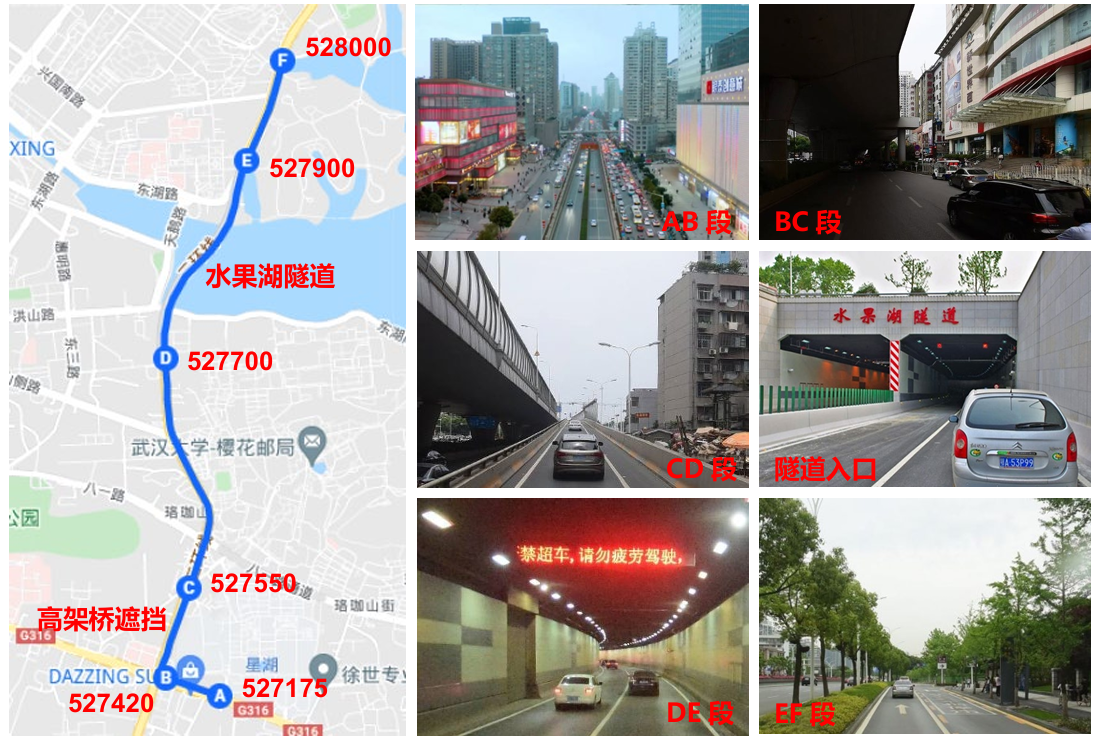
\includegraphics[width=0.65\textwidth]{figures/数据采集.png}
    \caption{RANSAC方法数据采集示意图}
    \label{ransac-data}
\end{figure}
相关的定位相关解算结果如下:
\begin{figure}[H]
    \centering
    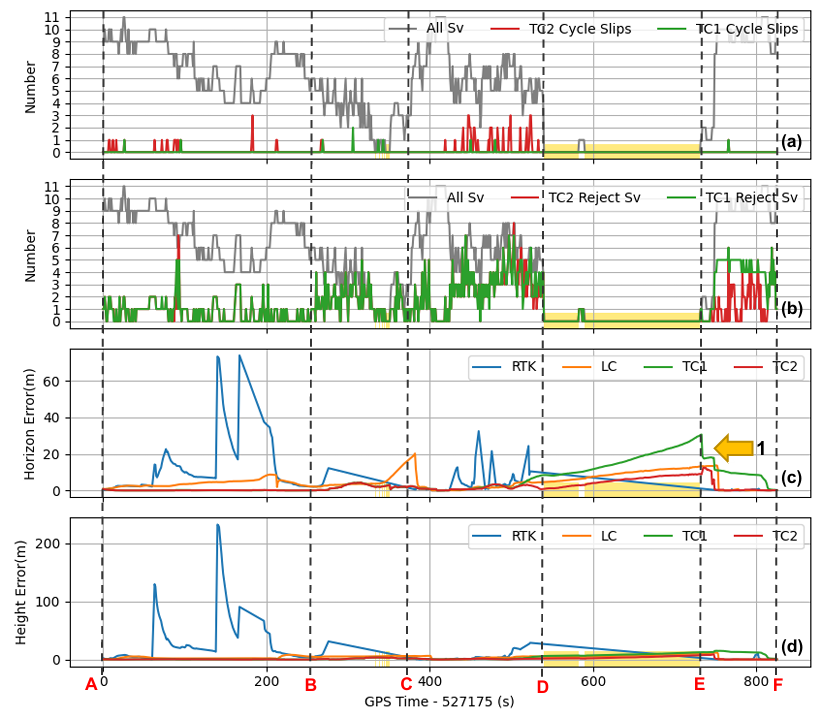
\includegraphics[width=0.8\textwidth]{figures/数据采集1.png}
    \caption{(高楼-高架桥-隧道) RTK、LC、TC1、TC2模式的位置误差、卫星数量与
    紧组合抗差细节 (子图横轴金色覆盖部分表示该区间无GNSS信号)  }
    \label{ransac-data1}
\end{figure}

从图\ref{ransac-data1}可知,TC2的位
置精度高于TC1与LC;TC1的北向位置误差较大,主要是由于在隧道前后路段
没有正确剔除粗差。该实验中GNSS信号中断时间较长,RTK定位成功率不足50\%,
松组合虽然能够保持连续定位,但是误差较大,定位有效率 (<5m) 只有33\%。
紧组合有效率突破60\%;TC2相比于TC1,有效率和固定率分别提高29\%和19\%。

\section{总结与展望}

随着全球导航卫星系统(GNSS)技术的快速发展,其在城市环境中的应用日益广泛。然而,城市环境的复杂性给GNSS定位带来了前所未有的挑战,主要包括多路径效应、信号遮挡和电磁干扰等问题。这些问题严重影响了GNSS信号的接收和处理,进而影响了定位的精度和可靠性。本课程报告综述了近年来城市环境下GNSS抗差技术的研究进展,特别关注了多路径效应的抑制方法、信号遮挡的解决方案以及抗干扰技术的发展,并重点介绍了四种常见技术:最小二乘残差法、粗差拟准检定法、众数投票法和RANSAC方法。这些方法在提高GNSS定位精度和可靠性方面发挥了重要作用。

最小二乘残差法是一种基于统计假设检验的方法,它通过建立误差方程和最小二乘解,计算残差向量,并基于正态分布的性质,对残差进行标准化处理,以检测和剔除异常值。这种方法简单直观,适用于单次观测中的粗差检测,能够有效地识别和剔除含有粗差的观测值,从而提高定位结果的准确性。

粗差拟准检定法通过附加“拟准观测的真误差估值范数极小”的条件,解算真误差与观测量之间的秩亏方程组,求出真误差估值,并判断出可能存在的粗差。这种方法可以同时识别和定位多个粗差,并估计粗差的大小和精度,适用于复杂情况下的粗差处理。它在处理多历元粗差探测和剔除方面表现出色,能够有效地提高GNSS定位的可靠性。

众数投票法(Majority Voting)是在消电离层组合的码观测方程中,利用已知的精密卫星星历、卫星钟差和接收机位置的先验三维坐标,通过比较同一历元对不同卫星的接收机钟差,发现单历元粗差。这种方法算法简单,自动化程度高,能够有效地探测粗差并剔除含有粗差的观测值,进行最小二乘平差。

RANSAC方法是一种迭代方法,用于从包含异常值的数据中估计数学模型参数,特别适用于数据包含显著噪声或异常值时的鲁棒性拟合。RANSAC方法通过随机选择样本并计算共识集合,重复这一过程多次,并选择具有最大共识集合的模型参数作为最终模型。这种方法在GNSS抗差领域中,尤其是在高楼、高架桥、隧道等特殊情景下的定位质量分析中,显示出了其优越性。

尽管这些方法在城市环境下的GNSS抗差技术中取得了显著进展,但仍存在挑战和问题需要进一步研究和解决。未来的研究应重点关注以下几个方面:

\begin{enumerate}
    \item 多路径效应的精确建模:探索更为精确和高效的多路径效应建模方法,以更好地理解和预测多路径效应的影响。
    \item 信号遮挡情况下的高精度定位技术:继续研究先进的多传感器融合技术和辅助定位技术,以在信号遮挡情况下提供更高精度和可靠性的定位服务。
    \item 抗干扰技术的进一步优化:探索更为高效的自适应滤波技术、干扰检测与抑制技术和抗干扰天线设计,以在复杂电磁环境中提供更高精度和可靠性的定位服务。
\end{enumerate}

随着人工智能和机器学习技术的发展,将其应用于GNSS抗差技术的研究也显示出巨大潜力。通过机器学习算法对大量历史数据进行训练,可以提高多路径效应建模、信号遮挡预测和干扰检测的精度和效率。例如,文献中提出的基于机器学习的信号预测模型,通过对历史信号数据进行训练,在信号遮挡情况下实现了高精度的信号预测。未来的研究应进一步探索人工智能和机器学习技术在GNSS抗差技术中的应用,以提高定位精度和可靠性。

尽管近年来在城市环境下GNSS抗差技术取得了显著进展,但仍存在一些挑战和问题需要进一步研究和解决。未来的研究应重点关注多路径效应的精确建模、信号遮挡情况下的高精度定位技术以及抗干扰技术的进一步优化。同时,随着人工智能和机器学习技术的发展,将其应用于GNSS抗差技术的研究也具有重要意义。通过不断的探索和创新,GNSS在城市环境中的应用前景将更加广阔。

在未来的研究中,我们还需要关注以下几个方面:

\begin{enumerate}
    \item 算法的计算效率和实时性:随着城市环境的复杂性增加,GNSS抗差算法需要处理的数据量也在不断增加。因此,提高算法的计算效率和实时性是未来研究的重要方向。
    \item 算法的适应性和泛化能力:城市环境的多样性要求GNSS抗差算法具有很好的适应性和泛化能力。未来的研究应探索如何使算法能够适应不同的城市环境和不同的应用场景。
    \item 算法的集成和优化:将多种抗差技术集成在一起,并通过优化提高整体性能,是未来研究的另一个重要方向。这包括如何有效地结合不同方法的优点,以及如何平衡各种方法之间的性能和资源消耗。
    \item 实验和验证:未来的研究还需要更多的实验和验证,以评估不同抗差技术在实际城市环境中的表现。这包括在不同城市、不同天气条件和不同时间段进行广泛的测试。
    \item 跨学科合作:GNSS抗差技术的研究需要地理信息科学、电子工程、计算机科学等多个学科的知识和技术支持。未来的研究应加强跨学科合作,以促进GNSS抗差技术的发展。
\end{enumerate}

城市环境下的GNSS抗差技术是一个多学科、多技术交叉的领域,它的发展需要不断的技术创新和跨学科合作。随着技术的不断进步,我们有理由相信,GNSS在城市环境中的应用将更加广泛和深入,为人们的生活和工作带来更多便利。
\newpage
%%----------- 参考文献 -------------------%%
\bibliographystyle{unsrt}
\bibliography{reference}

\end{document}